\section{Blockchain}
\label{chapter:blockchain}

\textit{
  In dit hoofdstuk wordt de vraag  ``Wat is Blockchain technologie?" behandeld. Het betreft het vergaren van kennis over de basis van het Blockchain begrip waarbij er ingegaan wordt op wat Blockchain is en welke eigenschappen het heeft. Door het beantwoorden van deze vraag wordt er een definitie vastgesteld van Blockchain technologie die gebruikt wordt in het gehele verslag.
}

Een blockchain is een gedistribueerde database die bestaat uit een keten van in de computer of op internet vastgelegde en samengevoegde gegevens genaamd blocks. Om deze reden wordt blockchain technologie ook wel vergeleken met een grootboek. In zekere mate is dit correct maar het omschrijft niet het meest vooraanstaande aspect van blockchain, namelijk dat het gedecentraliseerd opereert.

Om de analogie voort te zetten; een grootboek is in handen van één organisatie waarin transacties van of naar de organisatie vastgelegd worden. Dit betekent dat er een centrale autoriteit is die kan bepalen of er überhaupt wel transacties plaatsvinden, of erger, het systeem buiten gebruik kan stellen. Daarnaast is de centrale autoriteit ook in staat misbruik te maken door bijvoorbeeld transacties te registreren naar de eigenaar van het grootboek. Dit brengt een risico met zich mee die blockchain technologie oplost door het grootboek te verspreiden over een netwerk dat ervoor zorgt dat deze centrale autoriteit niet meer nodig is.

Een traditionele blockchain is weergegeven in fig. \ref{blockchain_reference}. De keten van gegevens wordt bepaald door de volgorde waarin de gegevens zijn toegevoegd. Er is daarbij een eenvoudig te controleren systeem volgens welke voorafgaande blokken aan elkaar gerelateerd behoren te zijn. Door de inhoud van het vorige block crypto grafisch te versleutelen (ook wel hashen genoemd) en deze sleutel op te nemen in een opeenvolgend blok wordt ervoor gezorgd dat gegevens van eerdere blokken niet meer gemuteerd kunnen worden. Wanneer dit wel gebeurt zou de ketting verbroken worden omdat er een nieuwe sleutel gegenereerd wordt en opeenvolgende blokken zullen refereren naar een foutieve sleutel.
  
\begin{figure}[h]
  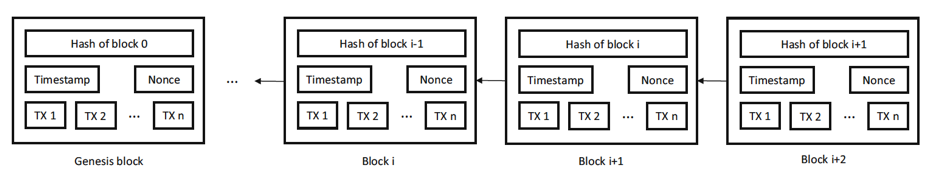
\includegraphics[width=1\textwidth]{figures/blockchain}
  \caption{Voorbeeld van een blockchain \citep{zheng2016blockchain}}
  \label{blockchain_reference}
\end{figure}

\clearpage
\subsection{Eigenschappen}

\cite{zheng2017overview}[Key Characteristics of Blockchain, p.5] stelt dat er vier eigenschappen zijn die een Blockchain definiëren:

\paragraph{Decentralisatie} In traditionele gecentraliseerde transactie systemen wordt iedere transactie gevalideerd door een centrale vertrouwde organisatie (e.g.\ banken), waardoor er een bottleneck gecreëerd wordt door de transacties te verwerken door centrale informatiesystemen. In contrast daarmee is een derde partij niet meer nodig in blockchain systemen. Consensus algoritmes zorgen ervoor dat data consistent is binnen het netwerk.

\paragraph{Persisentie} Transacties kunnen snel gevalideerd worden en invalide transacties zullen niet toegelaten worden. Het is bijna onmogelijk om te transacties verwijderen of ongedaan te maken als ze zijn opgenomen in de blockchain.

\paragraph{Anonimiteit} Elke gebruiker van het systeem kan interacteren zonder zijn ``echte" identiteit kenbaar te maken.

\paragraph{Controleerbaarheid} In bitcoin wordt de balans van een gebruiker opgeslagen door gebruik te maken van het Unspent Transaction Output (UTXO) model. Elke transactie refereert naar eerdere unspent transacties. Wanneer de huidige transactie is opgenomen in de blockchain, zal de staat van alle gerefereerde transacties verandert worden van ``unspent" naar ``spent". Hierdoor zijn transacties makkelijk te valideren en te traceren.